\documentclass[monografia]{subfiles}

\begin{document}

\chapter{Desenvolvimento}
	Neste capítulo é apresentado o processo de desenvolvimento do core de detecção de tons, abordando as 
	metodologias de desenvolvimento e teste, assim como explicação detalhada dos blocos pertencentes
	ao projeto, apresentando funcionalidades e de que maneira se comunicam com outros blocos de hardware.

	O core proposto foi projetado para ser inserido em um sistema, no qual, ele será responsável pelo processamento matemático
	dos áudios de sinalização monotônicos, de forma que ele é um elemento controlado por esse sistema.


\section{Metodologia de Desenvolvimento}
	Para o desenvolvimento deste trabalho foi aplicada a abordagem top-down, a qual se consiste em iniciar o desenvolvimento
	a partir dos blocos mais externos, baixando o nível de desenvolvimento até os blocos mais internos. Seguindo essa abordagem, 
	o desenvolvimento seguiu a ordem: \textit {Top Module; Tone Detector; Command Handler; Memory Control Access; Memory; 
	Signal Process; Message Handler} e \textit {Message Buffer}. 


\section{Ambiente de Desenvolvimento}
	Pelo fato deste trabalho ser desenvolvido tendo como alvo uma FPGA, o ambiente de desenvolvimento utilizado 
	foi o software \textit{Integrated Software Environment} (ISE) 14.7, tendo como hardware alvo a FGPA XC6VLX240T, da família virtex 6.
	Tanto o ambiente de desenvolvimento, quanto a FPGA são produzidos pela \textit{Xilinx}.

\section{Parâmetros da Detecção}
\label{sec:detectionParametersSection}
	Os áudios detectados pelo core apresentado neste trabalho são sinais monotônicos, que podem ser compostos por intercalações
	de pulsos e pausas. Os áudios também podem ter repetições de sequências de pulsos e pausas, essa característica é chamada de
	cadência. Essas características podem ser  melhor visualizadas na Figura \ref{fig:audioToneParameters}.

		\begin{figure}[!h]
		\centering 
		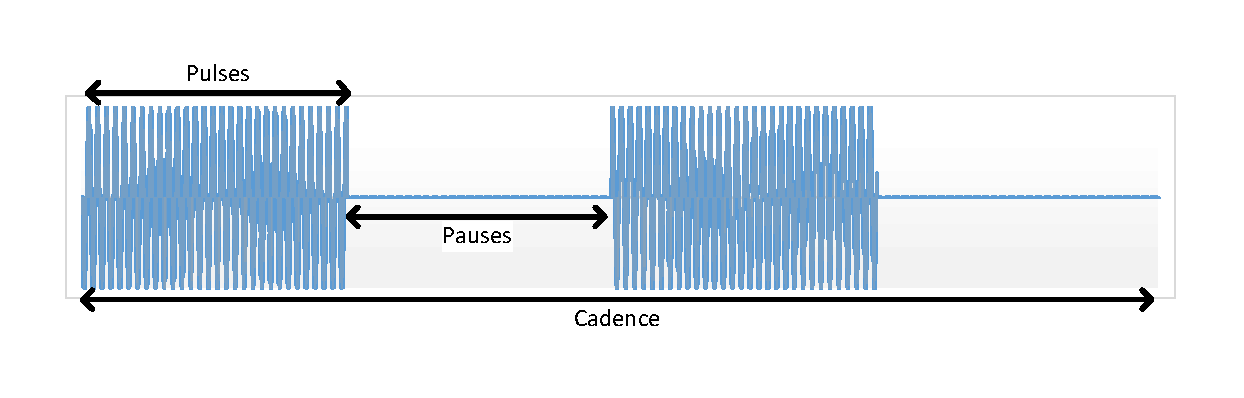
\includegraphics[scale=0.8]{img/audios/toneParameters.pdf}
		\caption{Pulsos, Pausas e Cadência}
		\label{fig:audioToneParameters}
		\end{figure}

	Para a detecção do áudio ser efetuada com sucesso, todos os parâmetros devem ser passados para o detector de tons. No total são 9 parâmetros,
	que detalham as características do áudio a ser detectado, são eles: \textit{MaxPulse}; \textit{MinPulse}; \textit{MaxPause}; 
	\textit{MinPause}; \textit{Attenuation}; \textit{Cadence}; \textit{Threshold}; \textit{Coeff1} e \textit{Coeff2}. Cada parâmetros está detalhado 
	a seguir.

	\begin{itemize}
	\item \textbf{MaxPulse e MinPulse}: Os primeiros parâmetros da detecção são relativos a duração de pulso do áudio. \textit{MaxPulse} e 
	\textit{MinPulse} são respectivos á duração máxima e mínima que o sinal deve ter. Estando o sinal processado fora desses limites, 
	implica que este áudio não está de acordo com o que se esperava, portanto, será entendido como áudio não detectado.
	\end{itemize}
	
	\begin{itemize}
	\item \textbf{MaxPause e MinPause}: Análogo aos parâmetros de duração de pulso, só que \textit{MaxPause} e \textit{MinPause} se referem à duaração das 
	pausas presentes no sinal. Entende-se como pausa, a parte do áudio que está presente o silêncio.
	\end{itemize}

	\begin{itemize}
	\item \textbf{Attenuation}:
		Dependendo da potência do sinal que estiver chegando na porta, talvez seja necessário fazer uma atenuação de cada amostra do sinal. A atenuação é 
		efetuada reduzindo a amplitude do sinal sempre em potências de dois. De acordo com a fórmula a seguir, onde, $S$ é a amostra que está chegando na 
		porta, e $S{a}$ é o valor da amostra atenuada.

			\begin{equation}
			S{a} = {S \over 2^{Attenuation}}
			\label{eq:SignalAttenuation}
			\end{equation}
	\end{itemize}

	\begin{itemize}
	\item \textbf{Cadence}: 
		A cadência é uma repetição de uma sequência de pulso e pausa. Na Figura \ref{fig:audioToneParameters} pode ser visto um sinal com cadência 0,
		ou seja, o sinal não tem repetição. Um exemplo de sinal com cadência é o tom de ocupado, utilizado na telefonia.
	\end{itemize}

	\begin{itemize}
	\item \textbf{Threshold}: Ao final do processamento de uma sequência de amostras, é feito o cálculo da sua potência, tendo este valor,
		temos que ter algum parâmetro que informe se esta potência refere-se a pulso ou pausa, este parâmetro de definição é o \textit{Threshold},
		que é o limiar utilizado para fazer tal classificação, que segue a seguinte lei:

			\begin{equation}
				\textit{Sequência} = \left\{\begin{array}{rc}
				pulso,&\mbox{se}\quad \textit{Potência} \ge Threshold,\\
				pausa, &\mbox{se}\quad \textit{Potência} < Threshold.
				\end{array}\right.
				\label{eq:ThresholdParameters}
			\end{equation}
	\end{itemize}

	\begin{itemize}
	\item \textbf{Coeff1 e Coeff2}:
		Estes parâmetros são relativos a frequência do áudio que se deseja detectar, \textit{Coeff1} e \textit{Coeff2} 
		informam para o detector de tons a faixa de frequência em que o sinal a ser processado deve estar presente. Neste trabalho proposto, 
		este intervalo é de $20 Hz$, ou seja, se o áudio a ser processado tem frequência igual $425 Hz$, os valores de \textit{Coeff1} e \textit{Coeff2}
		são correspondentes à $415 Hz$ e $435 Hz$. 

		Os valores dos coeficientes vêm da equação:
		\begin{equation}
			Coefficient = 2 \cos {\left ( \frac{2\pi f }{f_s} \right )}
			\label{eq:coeffCalc}
		\end{equation}

		Onde $f$ e $f_s$ são respectivamente a frequência desejada e a frequência de amostragem. Como na telefonia a frequência de amostragem dos
		sinais é $8 KHz$, a máxima frequência detectável é $4 KHz$, como pode ser provado no teorema da amostragem de Nyquist.
	\end{itemize}



\section{Desenvolvimento do Core}

%*********************************%
%*       TOP MODULE Section      *%	
%*********************************%
	\subsection{Top Module}
		A instância mais alta do projeto é o \textit{Top Module}, neste bloco, ficam instanciados o hardware que realmente será sintetizado,
		\textit{Tone Detector}, e também a unidade de testes, que é responsável pela inserção de comandos e áudios, assim como recebimentos
		de mensagens para análise dos resultados. A Figura \ref{fig:topModuleBlock} ilustra o \textit{Top Module}.


			\begin{figure}[!h]
			\centering 
			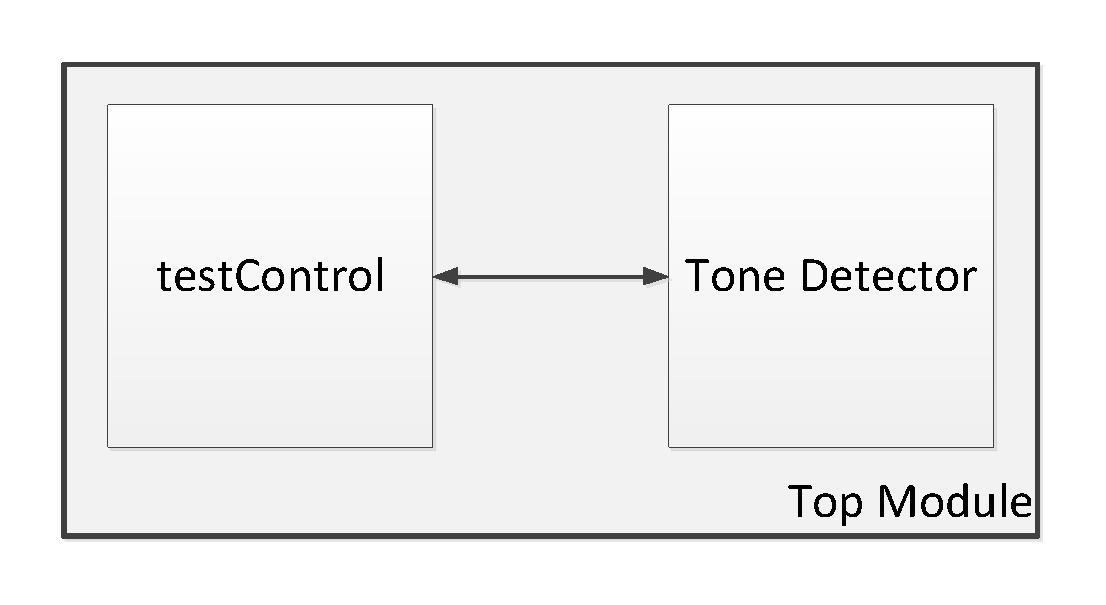
\includegraphics[scale=0.5]{img/modulos/mod_topModule.pdf}
			\caption{Top Module}
			\label{fig:topModuleBlock}
			\end{figure}

%*********************************%
%*     Tone Detector Section     *%	
%*********************************%
	\subsection{Tone Detector}
		O módulo \textit{Tone Detector}, assim com o \textit{Top Module}, é um bloco que somente instancia outros blocos, a diferença aqui é
		que este bloco instancia o Hardware a ser sintetizado. Dentro dele estão os módulos que são responsáveis por todo o processamento.
		O \textit{Tone Detector} é responsável por interligar as interfaces de comando, mensagens e áudio aos blocos responsáveis por cada 
		tarefa. A Figura \ref{fig:toneDetectorBlock} mostra uma visão geral deste módulo.

			\begin{figure}[!h]
			\centering 
			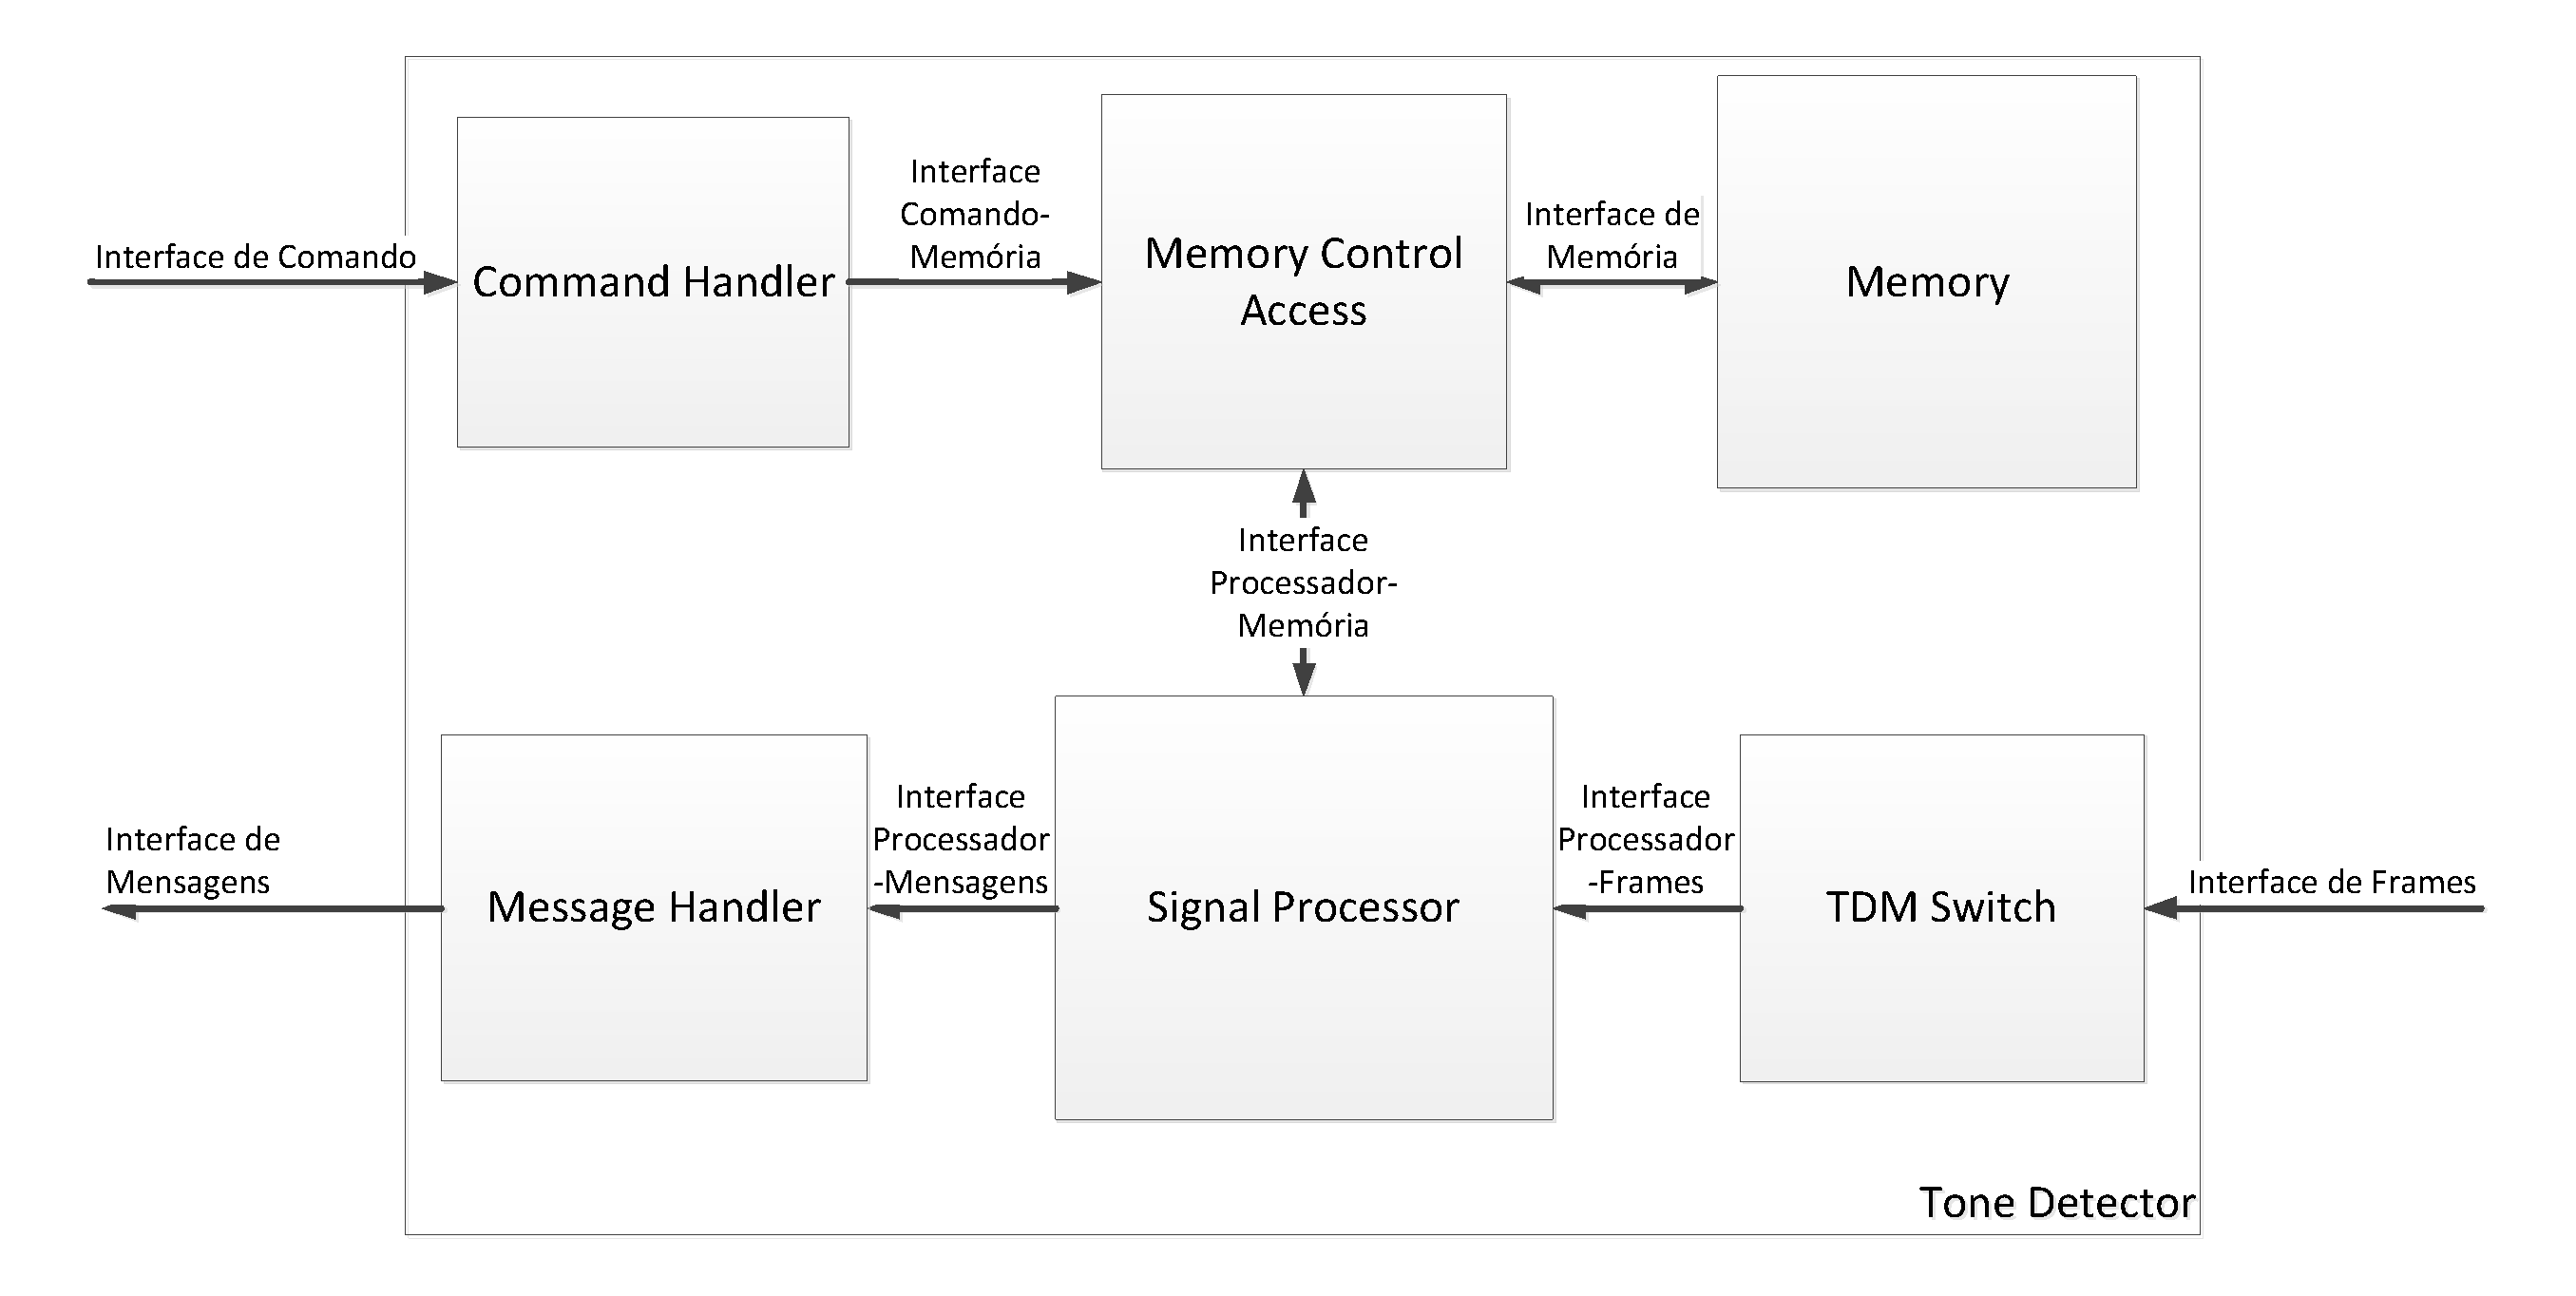
\includegraphics[scale=0.36]{img/modulos/modules_detail.pdf}
			\caption{Módulo Tone Detector}
			\label{fig:toneDetectorBlock}
			\end{figure}	

		Nas próximas Seções será detalhado cada bloco contido dentro do \textit{Tone Detector}, seguindo a sequência: 
		\textit{Command Handler; Memory Access Controller; Signal Processor e Message Handler}.



%*********************************%
%*    Comand Handler Section     *%	
%*********************************%
	\subsection{Tratamento dos Comandos}
		Para o processamento de um áudio ter seu início, os parâmetros da detecção para este áudio devem estar presente na região 
		de memória reservada para a porta na qual o tom irá ser detectado. A passagem dos parâmetros é feita através da interface de comando
		do \textit{Tone Detector}, esta interface está conectada com o bloco de hardware \textit{Command Handler}, que é responsável por decodificar
		a porta na qual será efetuada a detecção, e escrever na memória os parâmetros para tal detecção. 
		
		Internamente ao \textit{Command Handler}, existe um buffer de comando, no qual ficam armazenados os parâmetros, temporariamente, 
		até que o acesso à memória seja liberado pelo controlador de acesso à memória. O \textit{Command Buffer} é uma pequena 
		memória de 7x16 bits, a qual recebe os parâmetros para a detecção.  
		O módulo \textit{Command Handler} é representado pela Figura \ref{fig:commandHandlerBlock}, a seguir.

			\begin{figure}[!h]
			\centering 
			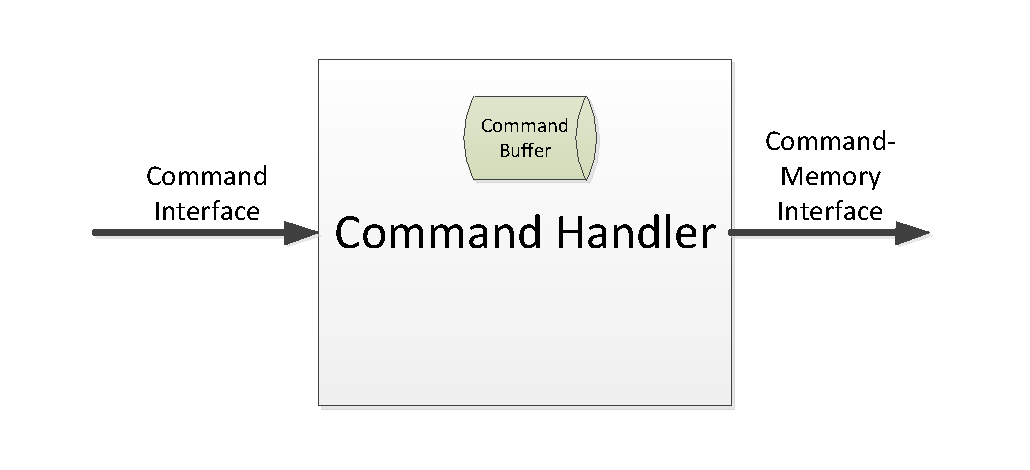
\includegraphics[scale=0.63]{img/modulos/mod_commandHandler.pdf}
			\caption{Command Handler}
			\label{fig:commandHandlerBlock}
			\end{figure}


		\subsubsection*{Command Handler}		
		\label{sec:commandHandlerSection}
			O módulo \textit{command handler} é responsável por receber os parâmetros do sinal a ser detectado e escrever esses parâmetros na memória. 
			À medida que cada parâmetro é recebidos, são escritos no \textit{command buffer}, para serem posteriormente escritos na memória.

			A comunicação na interface de comando é estabelecida através de um \textit{handshake}, onde primeiramente o controlador do core faz
			um pedido de requisição de envio dos parâmetros, após a requisição ser atendida, os mesmos serão enviados. A requisição, recebimento dos 
			parâmetros, armazenamento no \textit{command buffer} e escrita na memória seguem uma sequência, que está definida na máquina de estados
			do \textit{command handler}, que é representada pelo diagrama de máquina de estado na Figura \ref{fig:commandHandlerStatemachine}.

				\begin{figure}[!h]
				\centering
 				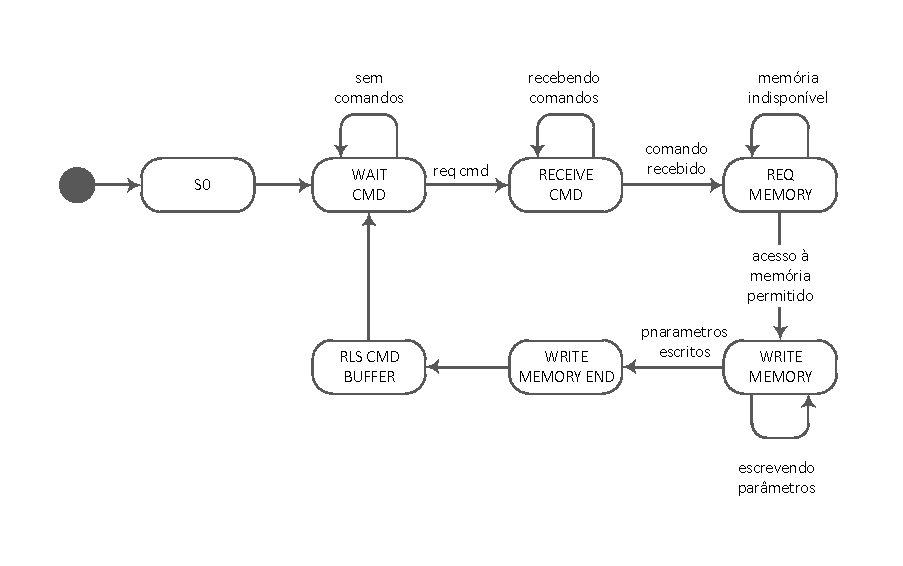
\includegraphics[scale=1.12]{img/stateMachines/commandHanlder.pdf}
				\caption{Máquina de Estados do Command Handler}
				\label{fig:commandHandlerStatemachine}
				\end{figure}

			O primeiro estado, \textbf{S0}, é o estado em que este módulo entra no reset do sistema, sua função é resetar os sinais contidos no 
			\textit{command handler}. Após o período de reset, a máquina avança para o estado  \textbf{WAIT\_CMD}, no qual 			
			fica esperando uma requisição de recebimento de comando. Enquanto não houver requisição, a máquina permanecerá no mesmo estado.

			Com o recebimento da requisição, o estado é alterado para \textbf{RECEIVE\_CMD}, dando início ao recebimento dos parâmetros, 
			contidos no comando. É recebido uma \textit{WORD} de 16 bits por vez, cada uma contendo um ou mais parâmetros. 
			A sequência, e a organização dos parâmetros dentro de cada \textit{WORD} é mostrada na 
			Figura \ref{fig:detectionParameters}:

				\begin{figure}[!h]
				\centering 
				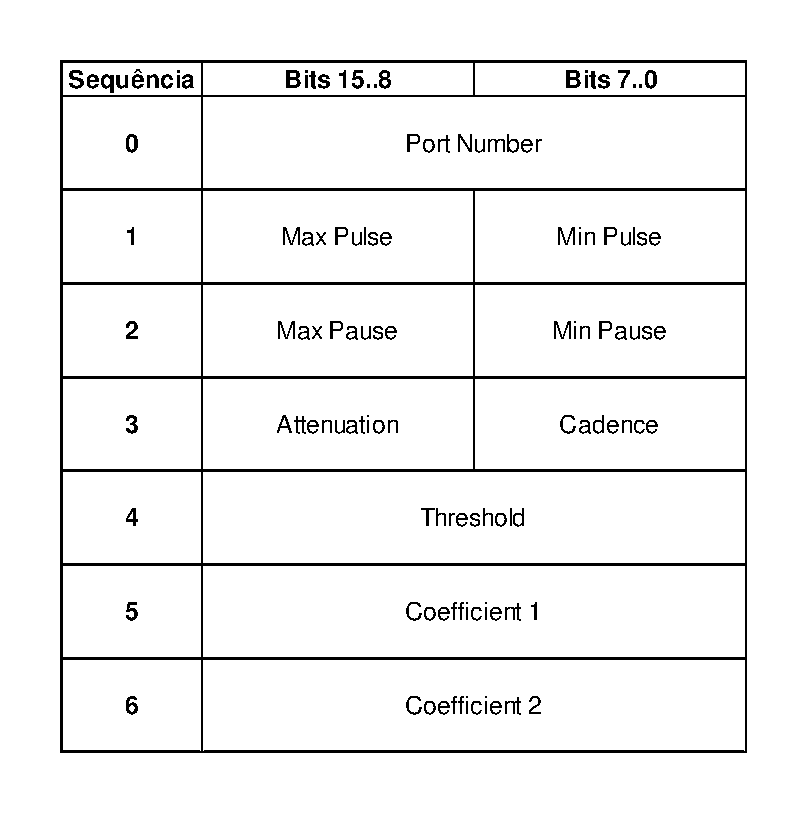
\includegraphics[scale=0.9]{img/memoryStructs/cmdBuffer.pdf}
				\caption{Parâmetros da Detecção}
				\label{fig:detectionParameters}
				\end{figure}



				% \begin{table}[]
				% \centering
				% \caption{Tabela de sequência de parâmetros}
				% \label{tab:parametersSequenceTable}
				% \begin{tabular}{|c|c|l|c|l|}
				% \hline
				% \textbf{Sequência} & \multicolumn{2}{c|}{\textbf{bits 15..8}} & \multicolumn{2}{c|}{\textbf{bits 7..0}} \\ \hline
				% \textbf{0}         & \multicolumn{4}{c|}{Port Number}                                                   \\ \hline
				% \textbf{1}         & \multicolumn{2}{c|}{Max Pulse}           & \multicolumn{2}{c|}{Min Pulse}          \\ \hline
				% \textbf{2}         & \multicolumn{2}{c|}{Max Pause}           & \multicolumn{2}{c|}{Min Pause}          \\ \hline
				% \textbf{3}         & \multicolumn{2}{c|}{Attenuation}         & \multicolumn{2}{c|}{Cadence}            \\ \hline
				% \textbf{4}         & \multicolumn{4}{c|}{Threshold}                                                     \\ \hline
				% \textbf{5}         & \multicolumn{4}{c|}{Coefficient 1}                                                 \\ \hline
				% \textbf{6}         & \multicolumn{4}{c|}{Coefficient 2}                                                 \\ \hline
				% \end{tabular}
				% \end{table}

			Após recebimento de todos os parâmetros, a máquina de estados avança para o estado \textbf{REQ\_MEMORY}, que é o estado responsável 
			por fazer a requisição de acesso à memória. O módulo responsável por atender esta solicitação é o \textit{Memory Access Controler}, 
			que será detalhado na Seção \ref{sec:memoryAccessControllerSection}.

			Com o acesso à memória liberado, acontece um avanço na máquina de estado, indo para o estado \textbf{WRITE\_MEMORY},
			iniciando assim a escrita dos parâmetros na memória. 
			Cada canal tem um espaço reservado na memória de 12 \textit{WORDS} de 16 bits, onde ficam contidos os parâmetros recebidos via comando,
			e outros parâmetros que são utilizados pelo \textit{Signal Processor}. O detalhamento de cada parâmetro e sua utilização será explanado
			na Seção \ref{sec:signalProcessSection}. 

			Com a escrita dos parâmetros finalizada, a máquina de estado do \textit{Command Handler} avança para o estado 
			\textbf{WRITE\_MEMORY\_END}. Esse estado fecha a conexão com a memória, fazendo com que ela esteja disponível no próximo ciclo de processamento
			do \textit{Signal Processor}. 

			Depois de concluída a escrita dos parâmetros, a máquina avança para o último estado, que é responsável por resetar 
			alguns sinais internos e o buffer de comando, o deixando pronto para receber um novo comando, esse estado é o 
			\textbf{RLS\_CMD\_BUFFER}. Após este reset, a máquina de estados do \textit{Command Handler} volta para o estado \textbf{WAIT\_CMD},
			assim ficando disponível para receber um novo comando. 
			Enquanto \textit{Command Handler} não voltar ao estado \textbf{WAIT\_CMD}, qualquer requisição de um novo comando, não será atendida.


	\subsection{Controle de Acesso à Memória}
	\label{sec:memoryAccessControllerSection}
		Devido ao acesso de memória poder ser requisitado por dois blocos de hardware, um controlador de acesso foi necessário, para que não houvesse
		uma política no acesso à memória. O bloco responsável por esse controle é \textit{Memory Access Control}, representado pela 
		Figura \ref{fig:memoryControlAccessBlock}.

			\begin{figure}[!h]
			\centering 
			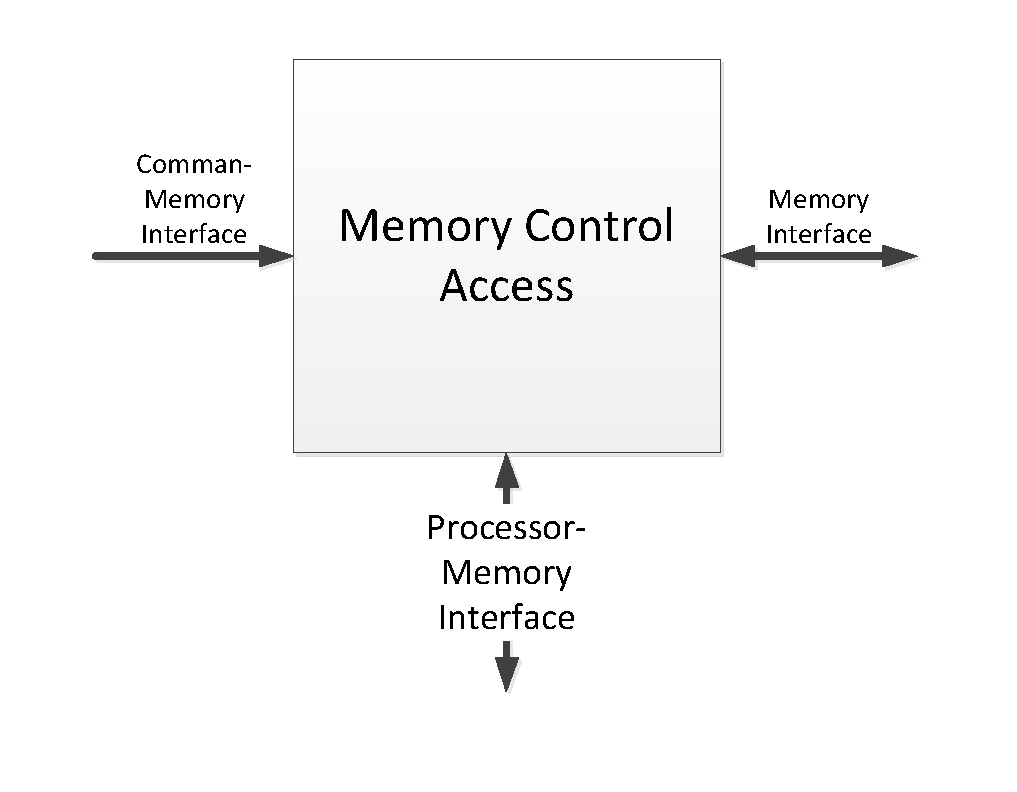
\includegraphics[scale=0.6]{img/modulos/mod_memoryControlAccess.pdf}
			\caption{Bloco de controle de acesso à memória}
			\label{fig:memoryControlAccessBlock}
			\end{figure}

		Este módulo tem seu funcionamento semelhante a um multiplexador, fazendo com que em alguns momentos o acesso à memória seja do processador de sinais,
		e em outros momentos este acesso seja do \textit{command handler}. 

		O funcionamento do \textit{Memory Access Control} é regido através de uma máquina de estados, que fica responsável por liberar o acesso à memória. 
		A máquina de estados do controle de acesso é apresentada na Figura \ref{fig:memControlAccessStatemachine}:

			\begin{figure}[!h]
			\centering
			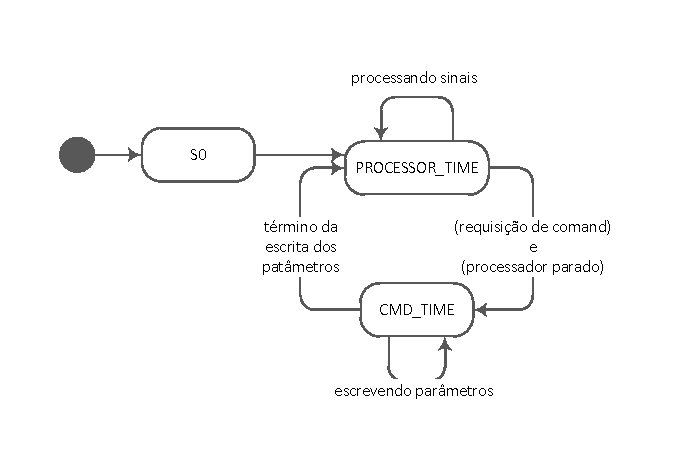
\includegraphics[scale=1.2]{img/stateMachines/memControlAccess.pdf}
			\caption{Máquina de Estado do Controle de Acesso à Memória}
			\label{fig:memControlAccessStatemachine}
			\end{figure}

		O estado inicial \textbf{S0} é o estado de \textit{reset}, sendo responsável por resetar os sinais internos do módulo, e deixando este apto para 
		seu funcionamento. Depois do reset dos sinais internos, a máquina de estado avança para o estado \textbf{PROCESSOR\_TIME}, que é o estado em que
		o acesso à memória fica sob o domínio do \textit{Signal Processor}. 

		Devido à maior prioridade que o processamento tem, em relação ao recebimento dos parâmetros vindos do \textit{command handler}, o controlador só
		libera o acesso da memória ao \textit{Command Handler} na ocorrência de dois eventos simultaneamente, o primeiro é se houver uma requisição do 
		\textit{command handler}, o segundo evento acontece quando o \textit{Signal Processor} não estiver processamento nenhum sinal, 
		neste momento o processador fica parado, esperando novas amostras. Esse comportamento do \textit{Signal Processor} 
		será explicado na Seção \ref{sec:HardwareStateMachine}. 

		Na ocorrência dos eventos citados, a máquina de estados avança para o estado \textbf{CMD\_TIME}, liberando assim o \textit{command handler} para
		efetuar escrita dos parâmetros para uma nova detecção. Ao final da escrita dos parâmetros a máquina de estados do \textit{Memory Access Control}
		retorna para o estado \textbf{PROCESSOR\_TIME}, assim disponibilizando a memória para o processador novamente.

		Devido ao fato de a memória ser acessada por dois blocos de hardware diferentes, tem que haver alguma margem de segurança para que não sejam criadas
		regiões críticas na memória. Esta margem é assegurada baseada no tempo em que o processador efetua suas operações na memória, pois, devido à velocidade
		com que acontece o processamento, existe tempo suficiente para tratar todos os oito canais e ainda receber comandos. Os detalhes dos tempos serão 
		apresentados na Seção \ref{sec:resultsSection}, que aborda e discute os resultados deste trabalho.
	
	% \subsection{Módulo de Demultiplexação no Tempo}

	\newpage

	\subsection{Memória}
	\label{sec:memoryorganizationSection}	

		Para que um áudio, que chega através de um canal de entrada, ser detectado corretamente pelo processador, é necessário que o mesmo
		esteja de acordo com os parâmetros da detecção passados via comando. Para validar se o áudio tem as características descritas de acordo com os
		parâmetros, são necessárias algumas variáveis controle. Ambos, parâmetros e variáveis de controle, de todos os canais, ficam na memória do 
		\textit{Tone Detector}. 

		Cada canal tem sua região na memória, são oito canais e cada região ocupa doze posições de dezesseis bits, portanto totalizando uma 
		memória de 96x16 bits de tamanho. A Figura \ref{fig:memoryOrganization} mostra a organização dos parâmetros e variáveis para cada canal de
		detecção.
			
			\begin{figure}[!h]
			\centering 
			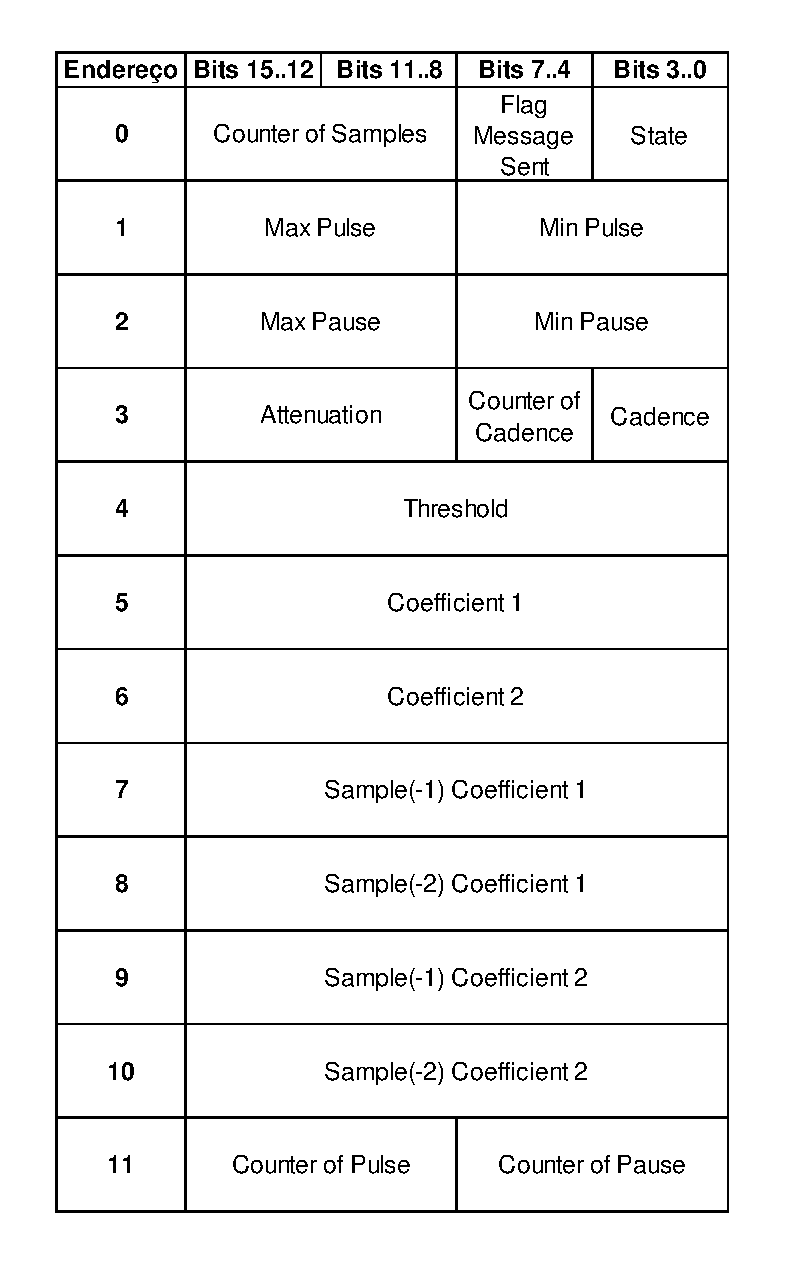
\includegraphics[scale=0.80]{img/memoryStructs/timeSlot.pdf}
			\caption{Organização da memória para cada canal}
			\label{fig:memoryOrganization}
			\end{figure}

		As variáveis de controle utilizadas no processamento dos áudios são: \textit{State}; \textit{Flag Message Sent}; \textit{Counter of Cadence};
		\textit{Sample(-1) Coefficient 1}; \textit{Sample(-2) Coefficient 1}; \textit{Sample(-1) Coefficient 2}; \textit{Sample(-2) Coefficient 2}; 
		\textit{Counter of Samples}; \textit{Counter of Pulses} e \textit{Counter of Pauses}. A seguir é mostrada a utilidade de cada variável.



		\begin{itemize}
		\item \textbf{State}: 
			Variável que guarda qual o estado da detecção em que o áudio está. São quatro estados possíveis, que são pertencentes 
			à máquina de estados da detecção, que será detalhada na Seção \ref{sec:detectionStateMachine}.
		\end{itemize}

		\begin{itemize}
		\item \textbf{Flag Message Sent}: 
			Flag que informa se a mensagem da detecção, sendo efetuada com sucesso ou não, foi enviada ao \textit{Message Handler},
			para através deste, ser enviada para o responsável por receber as mensagens do \textit{Tone Detector}.
		\end{itemize}

		\begin{itemize}
		\item \textbf{Counter of Cadence}: 
			Variável responsável por guardar a contagem de cadências que o sinal tiver ao longo da detecção. Essa variável só tem
			seu valor alterado quando o valor da cadência é maior que zero, ou seja, o sinal que será detectado tem repetições.
		\end{itemize}

		\begin{itemize}
		\item \textbf{Samples Coefficient}: 
			Por conta da utilização do algoritmo de Goertzel, que é usado para efetuar as detecções do 
			\textit{Tone Detector}, não é necessário guardarmos todas as amostras para verificar se uma frequência específica está presente no sinal, só é
			preciso guardar os dois últimos resultados. Este dois últimos resultado são respectivamente \textit{Sample(-1)} e \textit{Sample(-2)}. 
			Como o processamento acontece sempre com um cálculo do algoritmo de Goertzel para duas frequência, que são representadas pelos parâmetros 
			\textit{Coeff1} e \textit{Coeff2}, temos que guardar os dois últimos resultados para cada coeficiente, assim temos
			\textit{Sample(-1) Coefficient 1} e \textit{Sample(-2) Coefficient 1}, que são os últimos resultado para o primeiro coeficiente, e
			\textit{Sample(-1) Coefficient 2} e \textit{Sample(-2) Coefficient 2}, últimos resultados para o segundo coeficiente.
		\end{itemize}

		\begin{itemize}
		\item \textbf{Counter of Samples}:
			É a variável responsável por fazer a contagem de cada amostra de áudio que estiver chegando nos canais de recepção. Cada oitenta amostras 
			de sinal, que corresponde a $10 ms$ de áudio, equivale a um frame, que dependendo da potência pode ser pulso ou pausa. 
		\end{itemize}

		\begin{itemize}
		\item \textbf{Counter of Pulses}:
			Variável que guarda a quantidade de pulsos presentes no sinal que está sendo processado. A cada frame de áudio detectado, 
			esta variável tem seu valor incrementado de um. 
		\end{itemize}

		\begin{itemize}
		\item \textbf{Counter of Pauses}:
			Análogo à \textit{Counter of Pulses}, só que a variável \textit{Counter of Pauses} é responsável por fazer a contagem das pausas.
		\end{itemize}

	\newpage

	\subsection{Processador de Sinal}
	\label{sec:signalProcessSection}


	Nesta Seção é apresentado o principal bloco de hardware deste trabalho, o \textit{Signal Processor},  representado pela
	Figura \ref{fig:signalProcessorBlock}, é responsável por efetuar processamento
	dos áudios que chegam nos canais de entrada, verificar se a detecção ocorreu de acordo com os parâmetros recebidos e envio da mensagem ao módulo 
	de tratamento de mensagens, informando se a detecção aconteceu com sucesso, ou não. 

		\begin{figure}[!h]
		\centering 
		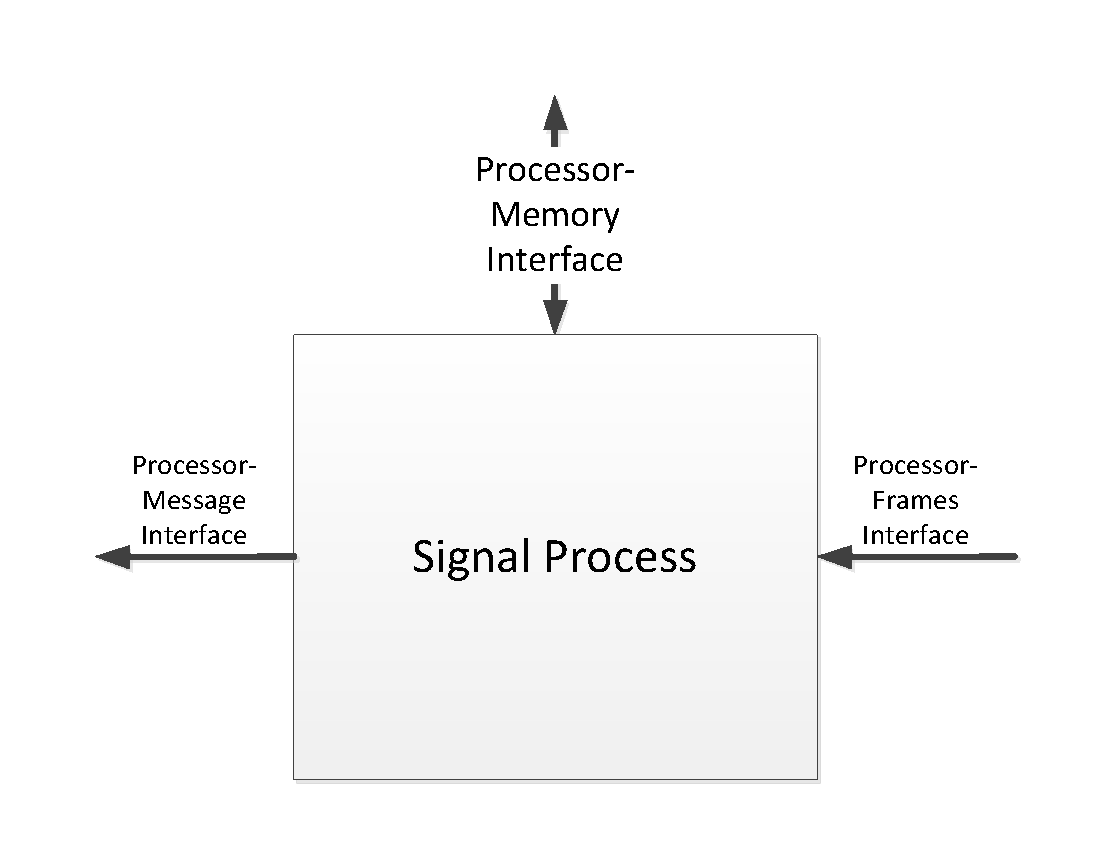
\includegraphics[scale=0.6]{img/modulos/mod_signalProcess.pdf}
		\caption{Bloco do Processador de Sinais}
		\label{fig:signalProcessorBlock}
		\end{figure}

	No módulo \textit{Signal Processor} existem duas máquinas de estado, que juntas realizam as tarefas pertinentes ao processamento dos sinais.
	A primeira é a máquina de estados da detecção, que determina em qual passo a detecção está, assim como a definição de quais os próximos passos, 
	sendo uma para uma para cada canal e estando as informações para seu funcionamento na região de memória de cada canal. Esta máquina tem quatro 
	estados, que são responsáveis por identificar se o sinal tem amplitude suficiente para ser processado, detectar pulsos, pausas e enviar mensagens.

	A segunda máquina de estado é a responsável pelo gerenciamento do hardware do \textit{Signal Processor}, esta é única para todos canais. Seu andamento é
	definido através de análise do estado atual, para cada canal, da máquina de estados da detecção. A máquina de estados do hardware é quem efetivamente
	lê da memória cada canal, efetua cálculos, verificações e envio de mensagens.

	Nas Seções \ref{sec:detectionStateMachine} e \ref{sec:HardwareStateMachine} serão detalhadas as máquinas de estados presentes no 
	\textit{Signal Processor}, demonstrando todos os estados, assim como que a máquina de estado da detecção influi no andamento da 
	máquina do hardware.


		\subsubsection{Máquina de Estados da Detecção}
		\label{sec:detectionStateMachine}		
			A máquina de estados da detecção, como dito antes, tem como papel gerenciar o processamento dos áudios. Cada canal de detecção tem sua própria
			máquina, pelo fato de que o processamento dos áudio são independentes entre si. Para tal gerenciamento, esta máquina é constituída pelos
			estados \textit{DT\_STATE0}, \textit{DT\_STATE1}, \textit{DT\_STATE2} e \textit{DT\_STATE3}, que de maneira resumida, são respectivamente responsáveis
			por verificar se o sinal em processamento tem amplitude necessária para início da detecção, detectar pulsos presentes no sinal, detectar intervalos
			de pausas e envio da mensagem da detecção, a Figura \ref{fig:detectionStatemachine} mostra o diagrama da máquina de estado da detecção. 

				\begin{figure}[!h]
				\centering
				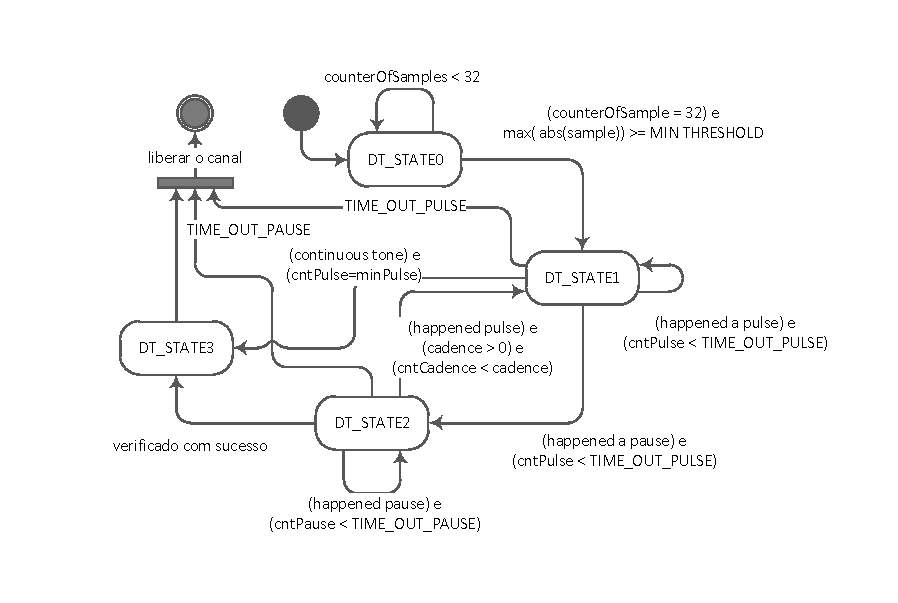
\includegraphics[scale=1.15]{img/stateMachines/dtState.pdf}
				\caption{Máquina de Estados da Detecção}
				\label{fig:detectionStatemachine}
				\end{figure}

			\subsubsubsection*{Estado da Detecção 0}
				\label{sec:dtState0Section}	
				Após o recebimento do comando, contendo os parâmetros da detecção, e a escrita destes na memória, o canal está pronto para iniciar a detecção 
				do áudio. O primeiro passo a ser feito no processamento do sinal, é a verificação das amplitudes das primeiras amostras, fazendo com que o
				processamento não seja iniciado até que um sinal contendo pulsos seja conectado na porta de entrada do canal.

				A verificação é feita após o recebimento de trinta e duas amostras consecutivas, o que equivale a $4 ms$ de áudio, sempre guardando na memória o módulo
				da amostra de maior valor absoluto. Após as trinta e duas amostras serem recebidas, pega-se a amostra armazenada na memória, fazendo a comparação desta 
				com a constante \textit{MIN\_THRESHOLD}. Se a amostra for maior ou igual, a máquina de estados avança para o estado  \textit{DT\_STATE1}, se não,
				permanece no estado  \textit{DT\_STATE0}, e refaz a verificação de mais trinta e duas amostras.
			
			\subsubsubsection*{Estado da Detecção 1}
				\label{sec:dtState1Section}
				Após constatar que o sinal é detectável, é dado início ao processamento dos pulsos presentes no áudio, que é efetuado no estado
				\textit{DT\_STATE1}. Para a detecção dos pulsos, é utilizado o algoritmo de \textit{Goertzel}, que faz o cálculo de uma DFT de forma iterativa,
				para uma única frequência, não necessitando guardar todas as amostras para o resultado final.	
				São necessárias 80 amostras de áudio para a detecção de um pulso, equivalendo a $10 ms$ de áudio. 

				A máquina de estados da detecção permanecerá no estado \textit{DT\_STATE1}, contabilizando pulsos enquanto não acontecer um \textit{timeout}.
				O valor de \textit{timeout} está definido na constante, definida em tempo de projeto, \textit{TIME\_OUT\_PULSE}, que tem
				valor igual a $250$ pulsos, ou seja, um áudio que tiver uma sequência de pulsos maior ou igual a $2500 ms$, terá sua detecção interrompida, 
				e será enviada uma mensagem indicando que aconteceu um \textit{timeout} de pulso.
			 	Não acontecendo \textit{timeout}, existe duas possibilidades para a saída do estado \textit{DT\_STATE1}.
			 	
			 	A primeira possibilidade é se ao decorrer da contabilização dos frames de pulsos, for detectado um frame de pausa. Se essa ação acontecer, 
			 	será incrementado o valor da variável \textit{Counter of Pauses}, e o estado será alterado para \textit{DT\_STATE2}, 
			 	que é o responsável por contabilizar os frames de pausas.

			 	A outra possibilidade é se o áudio for contínuo e a variável \textit{Counter of Pulses} e o parâmetro \textit{Min Pulse} forem iguais. 
			 	A informação de que um áudio é contínuo é passado através do parâmetro \textit{Min Pause}, se seu valor for zero, implica que 
			 	o áudio que se quer detectar não tem frames de pausas, Figura \ref{fig:continuousPulse}. 

			 		\begin{figure}[!h]
					\centering
						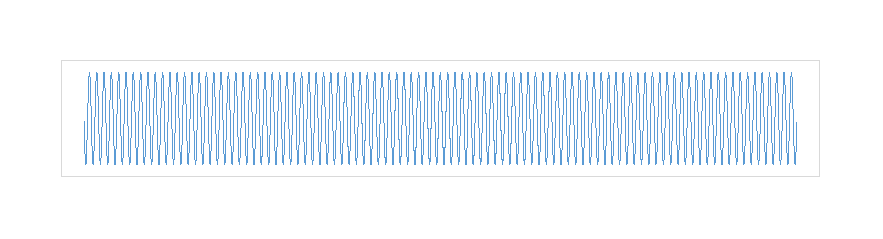
\includegraphics[scale=1.15]{img/audios/pulsoCont.pdf}
					\caption{Pulso Contínuo}
					\label{fig:continuousPulse}
					\end{figure}

			 	Sendo o sinal contínuo, só é necessário que o valor de \textit{Counter of Pulses}
			 	se iguale a \textit{Min Pulse}. Se isso ocorrer, o sinal é considerado detectado e o próximo estado será \textit{DT\_STATE3}, que é o estado
			 	responsável por enviar a mensagem de detecção.


			\subsubsubsection*{Estado da Detecção 2}
				\label{sec:dtState2Section}
				O estado \textit{DT\_STATE2} é o análogo ao estado \textit{DT\_STATE1} para as pausas. O cálculo matemático efetuado também é o 
				algoritmo de \textit{Goertzel}, diferenciando apenas, que nesse estado são contabilizadas as pausas. A maior diferença entre estes estados está
				na verificação, pois os únicos tipos de sinais que o \textit{DT\_STATE1} detecta são áudios contínuos, pois estes não precisam processar pausas. 
				Para ocorrer a detecção de todas as outras variações de sinais, é necessários que a máquina de estados passe pelo \textit{DT\_STATE2}.

				Depois de entrar no estado \textit{DT\_STATE2}, é iniciado o processamento das pausas e a variável \textit{Counter of Pauses} é incrementada
				para cada frame de pausa detectado, enquanto não houver um \textit{timeout} de pausas, esta variável  é incrementada. O valor do 
				\textit{timeout} de pausas é definido através da constante \textit{TIME\_OUT\_PAUSE}, que tem valor igual a duzentos, implicando em um intervalo de tempo
				de $2000 ms$. Igualmente ao \textit{DT\_STATE1}, se houver \textit{timeout} de pausa, a detecção é interrompida e uma mensagem de erro será enviada
				para sinalizar o erro ocorrido.	Estando a detecção no \textit{DT\_STATE2}, há três possibilidades de tipos sinais a serem 
				detectados: Sinais sem cadência com pausa contínua; Sinais sem cadência com pausa delimitada; Sinais com cadência. 
				Este são respectivamente representados na Figura \ref{fig:audioTypesDT2}. 

					\begin{figure}[!h]
					\centering
						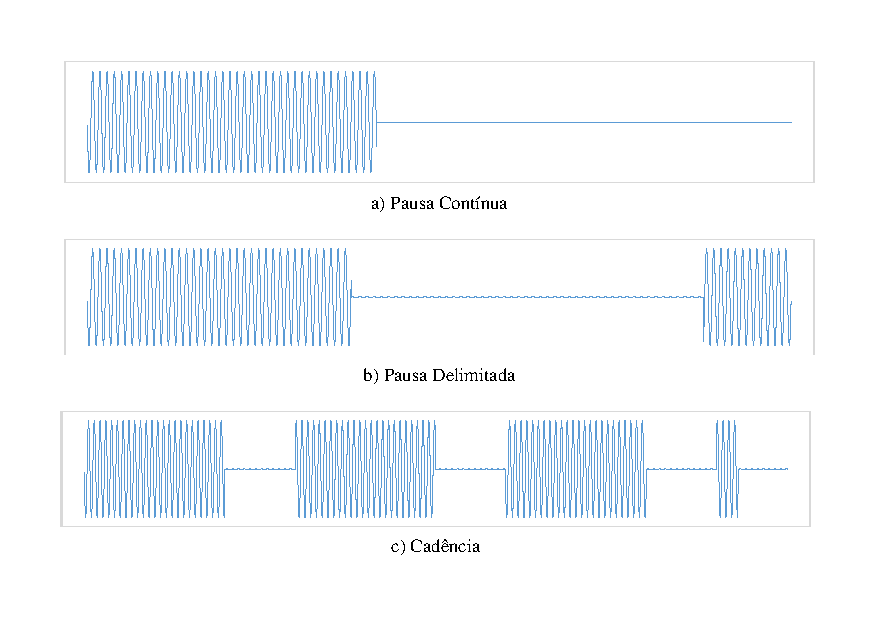
\includegraphics[scale=1.15]{img/audios/allTypesDTSTATE2.pdf}
					% \caption{Detectable Audios - DT\_STATE2}
					\caption{Áudios Detectáveis}
					\label{fig:audioTypesDT2}
					\end{figure}

				Áudios com pausa contínua, são aqueles em que não existe a necessidade de verificação da quantidade máxima de pausas contidas no sinal.
				O parâmetro \textit{Max Pause} é o responsável transmitir essa informação ao processamento, como pode ser visto na Eq. \ref{eq:PauseType}.

				 \begin{equation}
					Pausa = \left\{\begin{array}{rc}
					\textit{Contínua},&\mbox{se}\quad \textit{Pausa Máxima} = 0,\\
					\textit{Delimitada}, &\mbox{se}\quad \textit{Pausa Máxima} > 0.
				\end{array}\right.
				\label{eq:PauseType}
				\end{equation}

				% \newpage
				Para sinais com pausa, a contagem dos frames de pausa acontece até que o valor mínimo seja alcançado, ou seja, a variável \textit{Counter Of Pauses}
				tem seu valor incrementado até que seja igual ao parâmetro \textit{Min Pause}. Chegando a este ponto, o sinal é considerado como detectado, e máquina
				de estado avança para o estado \textit{DT\_STATE3}, para o envio da mensagem da detecção.
				
				Para áudios sem cadência, com pausa delimitada, sempre é esperado um frame de pulso após os frames de pausas, este pulso serve para informar ao
				processador que o período de pausa terminou. Após a chegada do pulso delimitador, o próximo passo é a verificação dos parâmetros de largura máxima
				e mínima dos pulsos e pausas. É dito que a detecção aconteceu com sucesso, se as variáveis \textit{Counter of Pulses} e \textit{Counter of Pauses}
				estiverem dentro dos limites máximos e mínimos, ou seja, $(Min Pulse \le CounterOfPulses \le Max Pulse)$ e 
				$(Min Pause \le CounterOfPauses \le Max Pause)$. Estando o sinal dentros dos limites especificados pelos parâmetros, este áudio é considerado
				detectado, e a máquina de estados avança para o estado \textit{DT\_STATE3}. Se os limites não forem respeitado, a máquina volta ao estado
				\textit{DT\_STATE1}, recomeçando o processamento.

				Um áudio com cadência é aquele composto por repetições de um sinal com pausa delimitada, ou seja, uma sequência de pulsos e pausas, como pode ser
				visto na Figura \ref{fig:audioTypesDT2}-c. Um sinal cadenciado faz a contagem dos frames de pulsos e pausas da mesma maneira, a diferença é que
				o pulso delimitador também é o início de uma nova sequência. Ao dar-se início a uma nova sequência, o valor da variável \textit{Counter of Cadence}
				é incrementado, \textit{Counter of Pulses} recebe o valor um, por se tratar do início de uma nova sequência,
				e \textit{Counter of Pauses} recebe o valor zero, e máquina de estado volta para o estado \textit{DT\_STATE1}, para o processamento dos novos pulsos.
				O sinal com cadência só será considerado detectado quando a variável \textit{Counter of Cadence} for igual ao parâmetro \textit{Cadence}, assim
				avançando a máquina de estados da detecção para o estado \textit{DT\_STATE3}, para o envio da mensagem de detecção.				

				% \newpage

			\subsubsubsection*{Estado da Detecção 3}
				\label{sec:dtState3Section}
				Quando a máquina de estados da detecção chega ao estado \textit{DT\_STATE3}, significa que a detecção do canal em questão foi concluída com sucesso,
				restando somente o envio da mensagem da detecção, que consiste em uma \textit{WORD} de 16 bits, dos quais, o byte mais significativo tem como valor a
				constante \textit{TS\_PROC\_SUCCESS}, que é definida em tempo de projeto, e neste trabalho está com o valor 0xAA. No byte menos significativo
				tem como valor a porta na qual a detecção foi efetuada, então, um exemplo de uma mensagem de detecção seria o valor 0xAA03, que expressa que o 
				áudio inserido no canal três foi detectado de acordo com os parâmetros passados via comando.			



		\subsubsection{Máquina de Estados do Hardware}
		\label{sec:HardwareStateMachine}
			A máquina de estado da detecção, como apresentado na Seção \ref{sec:detectionStateMachine}, é responsável pelo processamento de cada canal de
			áudio, abstraindo as operações de hardware que são necessárias para que a detecção aconteça com sucesso. 
			As operações de hardware são gerenciadas pela máquina de estados de hardware, Figura \ref{fig:hardwareStatemachine}, que é única para todos os canais.
			O hardware do \textit{Signal Processor} tem como funções: Leitura e escrita na memória; Cálculos matemáticos do algoritmo de \textit{Goertzel} e 
			Envio de mensagens. A seguir são explicados todas as ações e as lógicas de alternância de estado para esta máquina.

			\begin{figure}[!h]
			\centering
				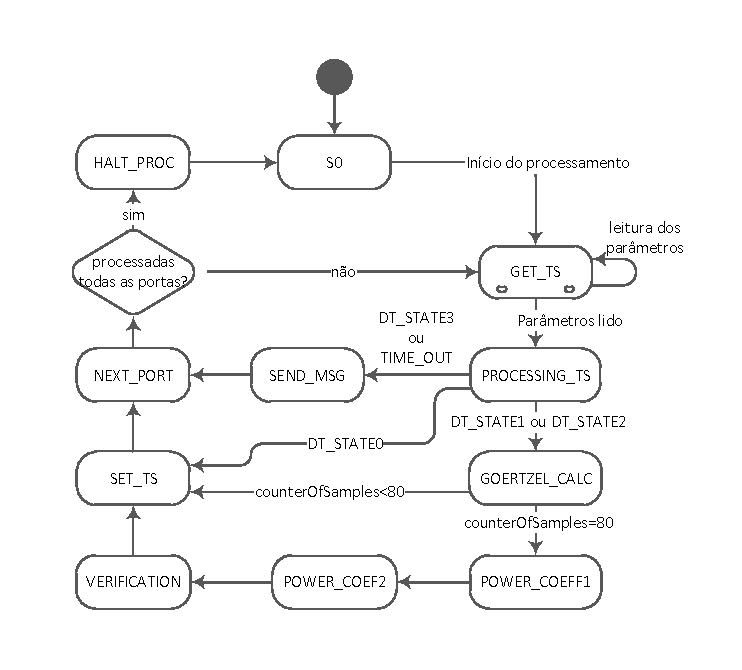
\includegraphics[scale=1.25]{img/stateMachines/hwProcState.pdf}
			\caption{Hardware State Machine}
			\label{fig:hardwareStatemachine}
			\end{figure}

			\subsubsubsection*{S0}
			\label{sec:hardwareStateS0}
				É o estado inicial da máquina de estados, responsável por resetar os sinais utilizados pelo hardware do \textit{Signal Processor}. A máquina
				permanece nesse estado apenas um ciclo de clock, avançando para o estado \textbf{GET\_TS}.

			\subsubsubsection*{GET\_TS}
			\label{sec:hardwareStateGETTS}
				O estado \textbf{GET\_TS} tem como objetivo fazer a leitura da região de memória de cada canal, para isso o \textit{Signal Processor} conta com
				um buffer interno de doze posições de dezesseis bits. Este buffer é utilizado para que durante o processamento de cada canal, não seja necessário fazer
				leituras ou escrita na memória. 

				Para não haver perca de tempo de processamento, o estado \textbf{GET\_TS} só lê toda a região de um canal, se o mesmo estiver sendo utilizado
				para algum processamento. A informação de que o canal não está processando consta no primeiro endereço de memória, dentro da região de memória
				de cada canal, se este valor for igual a 0xFFFF implica que este canal não está sendo usado para nenhuma detecção.

				Com o valor da primeira \textit{word} de posição de memória do canal diferente de 0xFFFF, inicia-se a leitura das \textit{words} restantes, 
				e a escrita deste valores no buffer interno. Com a leitura da memória do canal concluída, é dado início do processamento do canal, avançando a
				máquina de estados para o estado \textbf{PROCESSING\_TS}.

			\subsubsubsection*{PROCESSING\_TS}
			\label{sec:hardwareStatePROCESSINGTS}
				Este estado efetua um pré-processamento das informações lidas da memória, pertinentes ao canal que está sendo processado. Este pré-processamento
				define o próximo estado baseado no estado atual da máquina de estados da detecção do canal. Existem três estados possíveis para os quais a máquina 
				pode avançar: \textbf{SET\_TS}; \textbf{GOERTZEL\_CALC}; \textbf{SEND\_MSG}.

				A máquina de estados do hardware avança para estado \textbf{SET\_TS} se a máquina de estados da detecção, para o canal,
				estiver no estado \textit{DT\_STATE0}. Nessa situação é que acontece a coleta das primeiras amostras do áudio, como descrito na Seção 
				\ref{sec:dtState0Section}, na explicação do estado \textit{DT\_STATE0}.
				Após a coleta de uma amostra, é feita a comparação se esta tem magnitude maior que a amostra já guardada,
				nessa comparação sempre permanece a amostra de maior magnitude. Depois de guardada a maior amostra, a variável \textit{Counter of Samples},
				que faz a contagem das amostras, é incrementada. O estado \textbf{SET\_TS} é responsável por copiar a buffer interno para a  região de 
				memória do canal, isto é, escrever as alterações que foram feitas pelo processamento.

				Uma outra possibilidade de avanço de estado é para \textbf{GOERTZEL\_CALC}, para isto, o canal tem que está em fase de processamento de pulsos ou
				pausas, isto é, a máquina de detecção deste canal tem que está no estado \textbf{DT\_STATE1} ou \textbf{DT\_STATE2}, os quais fazem uso do algoritmo
				de \textit{Goertzel}, que é calculado no estado \textbf{GOERTZEL\_CALC}.

				O último estado possível de ser atingido através do \textbf{PROCESSING\_TS} é o estado \textbf{SEND\_MSG}, que é o responsável pela 
				geração e envio das mensagens, essa situação pode ser alcançada se a máquina de estado da detecção estiver no estado \textbf{DT\_STATE3},
				isto é, áudio processado com sucesso, ou se tiver acontecido um \textit{timeout} de pulsos ou um \textit{timeout} de pausas. 

			\subsubsubsection*{GOERTZEL\_CALC}
			\label{sec:hardwareStateGOERTZELCALC}
				Quando a máquina de estados do hardware chega a este estado, implica que frames de pulso ou de pausa estão sendo processados pelo canal de detecção,
				ou seja, quando a máquina de estado da detecção estiver nos estados \textbf{DT\_STATE1} ou \textbf{DT\_STATE2}, o algoritmo de 
				\textit{Goertzel} está sendo calculado para este canal. Este cálculo consiste de duas etapas, na primeira, é feito um cálculo em 
				oitenta amostras seguidas, equivalentes a $10 ms$ de áudio, e na segunda etapa é calculada a amplitude na frequência desejada.

				A etapa em que o algoritmo está é que decidirá o próximo estado da máquina de estado do hardware. A primeira etapa é sempre calculada para todas
				as amostras, e a segunda etapa de cálculo é feita na chegada da última amostra. O estado \textbf{GOERTZEL\_CALC} é responsável pelo cálculo da
				primeira etapa, e os estados \textbf{POWER\_COEFF1} \textbf{POWER\_COEFF2} efetuam os cálculos da segunda fase. Cada etapa é feita para os dois
				coeficientes de frequência, que são as variáveis \textit{Coefficient 1} e \textit{Coefficient 2}.

				O cálculo da primeira fase é realizado tendo os valores da amostra atual do áudio, \textit{Sample(0)}, e os dois últimos resultados do processamento,
				que estão salvos nas variáveis \textit{Sample(-1)} e \textit{Sample(-1)}. Para o cálculo é utilizada a variável auxiliar \textit{SampleAux}. 
				A expressão matemátiva para o processamento é apresentada a seguir.
				Este cálculo é feito para cada um dos coeficientes presente na memória.


				\begin{align}
					SampleAux & = Sample(0) + 2 \cdot Coefficient \cdot Sample(-1) - Sample(-2)\\
					Sample(-2) & = Sample(-1)\\
					Sample(-1) & = sampleAux
				\end{align}

				Quando efetuado o cálculo do octogésimo frame, nesse instante o valor da variável \textit{Counter of Samples} será igual a oitenta,
				a máquina de estados avança para o estado \textbf{POWER\_COEFF1}, e inicia o cálculo da segunda	etapa do algoritmo de \textit{Goertzel}.

				\newpage

			\subsubsubsection*{POWER\_COEFF1 e POWER\_COEFF2}
			\label{sec:hardwareStatePOWERCOEFF}

				Os estados \textbf{POWER\_COEFF1} e \textbf{POWER\_COEFF2} são responsáveis pelo cálculo das amplitudes das frequências correspondentes aos
				\textit{Coefficient 1} e \textit{Coefficient 2}, respectivamente. A principio esses cálculos poderiam ser realizados no mesmo estado, 
				sem alteração dos resultados, mas o resultado da ferramenta de síntese para o hardware da FGPA conseguiu um clock máximo de $20 MHz$. 
				Com os cálculos das amplitudes divididos em dois estados, um para cada coeficiente de frequência, a ferramenta conseguiu sintetizar
				o hardware com um clock máximo de $88.402 MHz$. 
				
				Com a primeira etapa do algoritmo de \textit{Goertzel} concluída, isto é, o processamento de oitenta amostras seguidas do áudio,
				a máquina de estado do hardware avança para o estado \textbf{POWER\_COEFF1}, e consequentemente para o estado \textbf{POWER\_COEFF2}.
				O resultado do cálculo das amplitudes para os dois coeficientes de frequência, 
				\textit{Coefficient 1} e \textit{Coefficient 2}, são escritos respectivamente em dois sinais internos do 
				\textit{Tone Detector}, que são \textit{POT1\_s} e \textit{POT2\_s}.
				A expressão matemática utilizada para o cálculo da potência para cada coeficiente é apresentado a seguir na equação \ref{eq:potRaia_1_2}.

				\begin{align}
				\label{eq:potRaia_1_2}
					Power & = Sample(-1)^{2} +  Sample(-2)^{2} -  2 \cdot Sample(-1) \cdot Sample(-2)
				\end{align}

				Com o cálculo das amplitudes concluído, a máquina de estados do hardware avança para o estado \textbf{VERIFICATION}, onde serão verificadas
				as variáveis de processamento do áudio, e que através de comparações destas com os parâmetros, será tomada a decisão do próximo passo da
				detecção, do canal que está sendo processado.



			\subsubsubsection*{VERIFICATION}
			\label{sec:hardwareStateVERIFICATION}
				Na Seção \ref{sec:dtState1Section} abordamos os estados \textit{DT\_STATE1} e 
				\textit{DT\_STATE2} da máquina de estados da detecção, estes estados, quando concluíam seus processamentos dos frames, seja de 
				pulso ou de pausa, iniciavam uma fase de verificação para, baseado no parâmetros da detecção, saber se o áudio havia sido 
				detectado ou não.  As transições que acontecem a partir dos estados \textit{DT\_STATE1} e \textit{DT\_STATE2} da máquina de 
				estados da detecção são decididas, a nível de hardware, no estado \textbf{VERIFICATION} da máquina de estados do hardware.

				\newpage

			\subsubsubsection*{SET\_TS}
			\label{sec:hardwareStateSETTS}
				Para o processamento de cada canal, é necessário copiar sua região na memória para o buffer interno. Com a cópia da memória efetua-se
				os devidos cálculos, incrementos e etc, mas todas as alterações são escritas no buffer interno, e não na memória do \textit{Tone Detector}.

				A escrita das alterações da região de memória, para cada canal, é efetuada no estado \textbf{SET\_TS}. É escrita uma \textit{WORD} de 
				dezesseis bits 
				em cada ciclo de clock, totalizando doze períodos de clock para a escrita de toda a região de cada canal de detecção.

			
			\subsubsubsection*{SEND\_MESSAGE}
			\label{sec:hardwareStateSENDMESSAGE}
				O estado \textbf{SEND\_MESSAGE} é responsável pelo envio das mensagens a nível de hardware, sejam mensagens de sucesso da detecção ou
				de ocorrência de \textit{timeout}. Em ambos os casos, após o envio da mensagem, a região de memória correspondente ao canal será liberada,
				para que esteja disponível para um novo processamento.

				Para a entrega da mensagem só é necessário verificar se ainda há espaço disponível no buffer de mensagens, esta verificação é feita
				através do sinal \textit{MSG\_BUF\_FULL}, sinal este que tem valor lógico baixo quando o buffer ainda tem espaço. 
				Este sinal vem diretamente do \textit{Message Handler}, que é o bloco de hardware
				responsável pelo envio das mensagens do \textit{Tone Detector}. Esta entrega da mensagem é efetuada em um único ciclo de clock, caso houver
				espaço, pois o
				\textit{Message Handler} está sempre esperando pelo recebimento de mensagens, isto faz com que não seja perdido tempo de processamento com
				a atividade de envio de mensagens. O bloco de hardware \textit{Message Handler} será detalhado na Seção \ref{sec:messageHandlerBlock}.



			\subsubsubsection*{NEXT\_PORT}
			\label{sec:hardwareStateNEXTPORT}
				A máquina de estados do hardware tem seu ciclo de execução para cada canal de detecção, durante este ciclo, ações como cálculos, leituras e
				escritas na memória, verificações e envio de mensagens podem ser feitas. Depois do processamento de um canal é iniciado o processamento do 
				próximo, se houver outro canal para ser processado. A mudança do canal a ser processado é feita pelo estado \textbf{NEXT\_PORT}.

				Se houver um próximo canal a ser processado, o valor do sinal interno \textit{port\_proc\_s}, que guarda o valor do canal de processamento atual,
				é incrementado e o próximo estado é \textbf{GET\_TS}, para a leitura da memória deste canal.

				Não havendo mais canais a serem processados, a máquina avança para o estado \textbf{HALT\_PROCESSOR}, fazendo com que o processador fique no aguardo
				por novas amostras de áudio para o processamento.

				\newpage

			\subsubsubsection*{HALT\_PROCESSOR}
			\label{sec:hardwareStateHALTPROCESSOR}
				Devido a frequência de amostragem dos áudios serem $8 KHz$, os sinais em detecção tem novas amostras de áudio disponível para processamento
				a cada $125 \mu s$. Com a frequência do clock do processador a $80 MHz$, todos os canais são processados muito antes que as novas amostras 
				estejam disponíveis. Neste tempo restante, o \textit{Signal Processor} interrompe seu processamento e libera a memória para que o bloco de
				hardware \textit{Command Handler}, Seção \ref{sec:commandHandlerSection}, tenha a memória disponível para que assim possa escrever parâmetros
				para um novo processamento.

				A máquina de estados do hardware permanece em \textbf{HALT\_PROCESSOR} até que novas amostras de áudio estejam disponíveis para o processamento,
				com isto, a máquina vai para o estado \textbf{S0}, e assim reinicia todo o ciclo de processamento.


	\subsection{Tratamento das Mensagens}
	\label{sec:messageHandlerBlock}
		A última interface do \textit{Tone Detector} é a de mensagens, estas representam as respostas aos processamentos iniciados através
		do \textit{Command Handler}, Seção \ref{sec:commandHandlerSection}. No bloco de hardware \textit{Message Handler}, Figura \ref{fig:messageHandlerBlock},
		está todo o processo de recebimento das mensagens do \textit{Signal Processor} e o envio destas através da interface de mensagens, ambas ações
		realizadas por duas máquinas de estados que são, respectivamente, a máquina de estados de recepção e a máquina de estados de transmissão de mensagens.

			\begin{figure}[!h]
			\centering 
			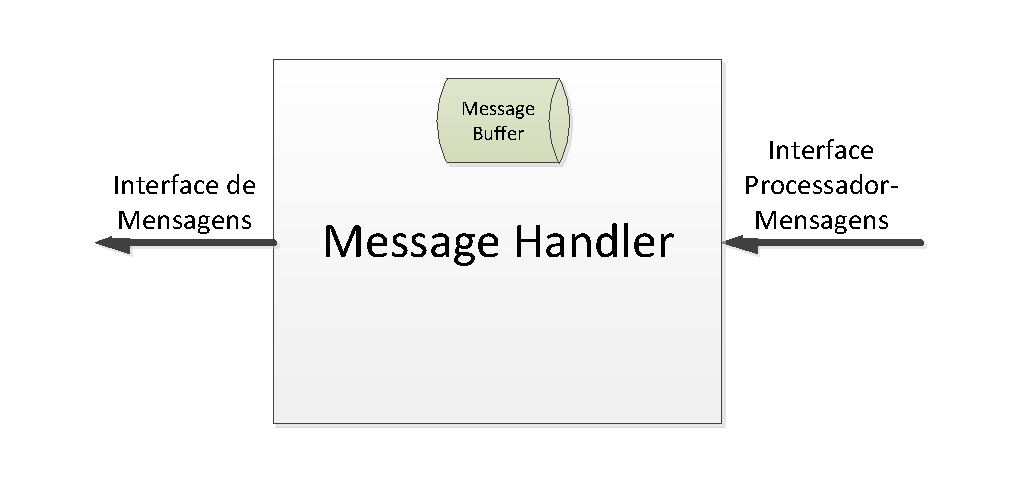
\includegraphics[scale=0.65]{img/modulos/mod_messageHandler.pdf}
			\caption{Message Handler Block}
			\label{fig:messageHandlerBlock}
			\end{figure}		

		As duas máquinas de estados fazem uso de um recurso comum, um buffer circular do tipo FIFO, para armazenar as mensagens da detecção, 
		para que as mesma possam ser enviadas via interface de mensagem. O acesso ao buffer circular é feito através de dois ponteiros, 
		que são os sinais internos \textit{buf\_tail\_s} e \textit{buf\_head\_s}, que respectivamente apontam para o para final e início da fila.
		As duas máquinas de estados serão explicitadas nos itens, a seguir.

		\subsubsection*{Rx State Machine}
		\label{sec:rxStateMachineSection}
			A máquina de estado de recepção de mensagens é constituída por cinco estados, que são: \textbf{S0}; \textbf{WAIT\_RX}; \textbf{RECEIVE\_DATA}; 
			\textbf{INC\_TAIL}; \textbf{WAIT\_FREE\_SPACE}. O diagrama de máquina de estados é mostrado na Figura \ref{fig:rxMessageStatemachine}.

			\begin{figure}[!h]
			\centering
				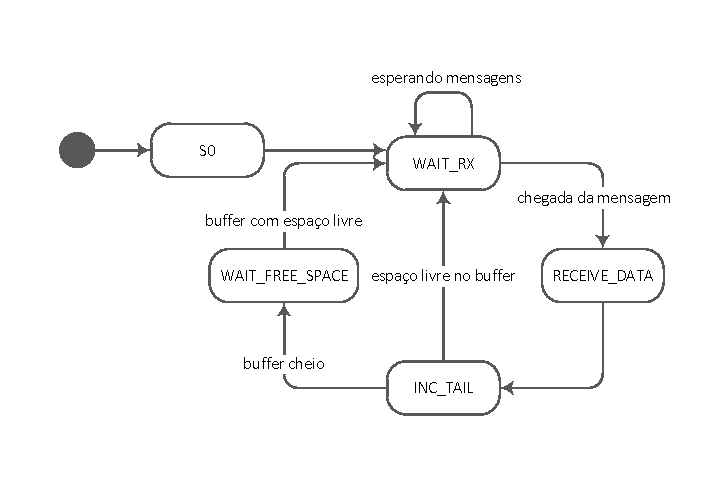
\includegraphics[scale=1.3]{img/stateMachines/rxMsgState.pdf}
			\caption{Rx Message State Machine}
			\label{fig:rxMessageStatemachine}
			\end{figure}

			No estado inicial, \textbf{S0}, são efetuado os resets dos sinais internos relativos a recepção das mensagens, assim como dos campos do buffer interno
			de mensagens. Após o período de reset, a máquina avança para o estado \textbf{WAIT\_RX}, e permanece deste modo enquanto o \textit{Signal Processor}
			não enviar nenhuma mensagem.

			Com a chegada da mensagem vinda do \textit{Signal Processor}, a máquina avança para o estado \textbf{RECEIVE\_DATA}, que salva o conteúdo da 
			mensagem no campo do buffer interno apontado pelo sinal interno \textit{buf\_tail\_s}, e após isso, a máquina avança para o 
			estado \textbf{INC\_TAIL}, neste estado, é efetuado o incremento ponteiro \textit{buf\_tail\_s}. Por se tratar de um buffer circular, um incremento 
			para quando \textit{buf\_tail\_s} estiver apontando para o final do buffer implica que ele irá apontar para o início  do buffer. A forma de
			incremento do ponteiro está apresentado em \ref{eq:bufTailIncrement}.

				\begin{equation}
					{buf\_tail\_s} = \left\{\begin{array}{rl}
					{buf\_tail\_s}+1,&\mbox{se}\quad {buf\_tail\_s} < {MSG\_BUFFER\_SIZE},\\
					0, &\mbox{alhures.}\quad
				\end{array}\right.
				\label{eq:bufTailIncrement}
				\end{equation}

				\newpage

				Após incremento, a máquina tem duas possibilidades de avanço de estado, retornar para \textbf{WAIT\_RX} se houver espaço no buffer, 
				e assim ficar na espera por novas mensagens, ou 
				ir para o estado \textbf{WAIT\_FREE\_SPACE} se não houver mais espaço disponível para armazenar mensagens no buffer interno.
				A máquina de estados de recepção de mensagens sabe que não tem mais espaço no buffer interno quando, após o incremento do ponteiro 
				\textit{buf\_tail\_s}, seu valor seja igual ao ponteiro \textit{buf\_head\_s}, que é o ponteiro que aponta para o início da fila.

				Chegando ao estado \textbf{WAIT\_FREE\_SPACE}, permanecerá até que \textit{buf\_tail\_s} e \textit{buf\_head\_s} tenham valores diferentes.
				Enquanto  estiver nesse estado, o sinal \textit{MSG\_BUF\_FULL} permanecerá em nível lógico alto, informando para o \textit{Signal Processor}
				que não há espaço para receber mensagens. Ao ser liberado espaço no buffer interno, a máquina retorna ao estado \textbf{WAIT\_RX}.
				

		\subsubsection*{Tx State Machine}
		\label{sec:txStateMachineSection}
			O último passo do processamento de um áudio é transmitir a informação de sucesso, ou não, da detecção para o módulo que estiver controlando 
			o \text{Tone Detector}. Se houver mensagem a ser transmitida, esta é enviada ao controlador externo via protocolo \textit{handshake}.
			A máquina de estados de transmissão de mensagens possue quatro estados, que são: \textbf{S0}; \textbf{WAIT\_MSG}; \textbf{SEND\_TX}; \textbf{INC\_HEAD}.
			O diagrama de máquina de estados está apresentado na Figura \ref{fig:txMessageStatemachine}.


			\begin{figure}[!h]
			\centering
				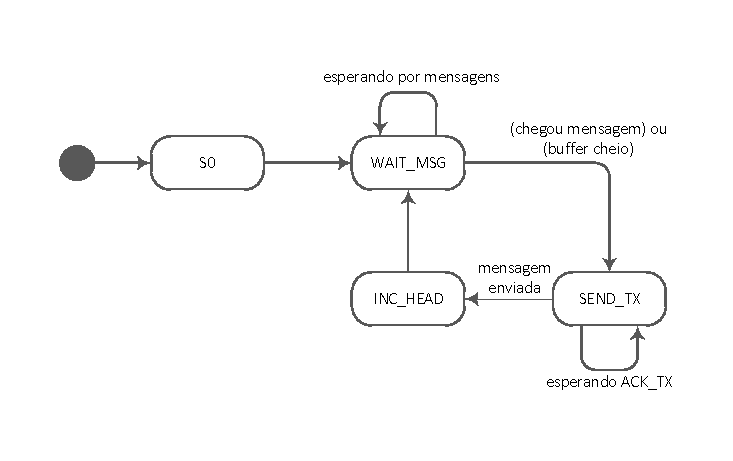
\includegraphics[scale=1.3]{img/stateMachines/txMsgState.pdf}
			\caption{Tx Message State Machine}
			\label{fig:txMessageStatemachine}
			\end{figure}

			\newpage

			O primeiro estado, assim como em todas as máquinas de estados deste trabalho, é o \textbf{S0}, o qual faz o reset dos sinais internos relativos
			a transmissão de mensagens do módulo \textit{Message Handler}. Após período de reset, a máquina avança para o estado \textbf{WAIT\_MSG}, onde
			permanece até que tenha alguma mensagem no buffer interno para envio, isto acontece quando \textit{buf\_tail\_s} e \textit{buf\_head\_s}
			possuem valores diferentes, ou quando o sinal \textit{MSG\_BUF\_FULL} tiver valor lógico alto.

			Com a existência de alguma mensagem para ser enviada, a máquina avança para o estado \textbf{SEND\_TX}.
			Nesse estado, é enviado um sinal de \textit{RX} ao controlador externo e a mensagem fica disponível para ser lida através do 
			sinal \textit{MSG\_TX\_DATA}. A máquina permanece nesse estado até receber uma resposta através do sinal \textit{ACK\_TX}, informando
			que o conteúdo da mensagem foi lido.

			Com a mensagem lida, a máquina avança para o estado \textbf{INC\_HEAD}, onde o valor do ponteiro \textit{buf\_head\_s} é incrementado. A forma de
			incremento deste ponteiro segue o mesmo protocolo de incremento para o ponteiro \textit{buf\_tail\_s}, como pode ser visto a seguir em 
			\ref{eq:bufHeaderIncrement}.

				\begin{equation}
					{buf\_header\_s} = \left\{\begin{array}{rl}
					{buf\_header\_s}+1,&\mbox{se}\quad {buf\_header\_s} < {MSG\_BUFFER\_SIZE},\\
					0, &\mbox{alhures.}\quad
				\end{array}\right.
				\label{eq:bufHeaderIncrement}
				\end{equation}

			Com o incremento do ponteiro concluído, a máquina de estados da transmissão de mensagens retorna ao estado \textbf{WAIT\_MSG}, assim ficando 
			disponível para envio de novas mensagens.

			\newpage



	\subsection{Unidade de Testes}
		\label{sec:testUnitySection}
			Com o desenvolvimento do \textit{Tone Detector} finalizado, foi necessário criar uma unidade de testes para validar a funcionalidade do 
			hardware proposto. A unidade de testes também está desenvolvida na linguagem VHDL, mas diferente do projeto do \textit{Tone Detector},
			utiliza funcionalidades que não são sintetizáveis, como leitura de arquivos. A unidade de testes aqui está descrita de maneira mais funcional,
			e portanto mais simplificada.

			A unidade de teste é composta por três módulos controlados, \textit{frameInserter}, \textit{commandInserter} e \textit{messageReceive},
			que respectivamente são responsáveis pela inserção dos comandos, inserção dos áudios, recepção das mensagens, 
			e um módulo controlador, \textit{testControl}, que gerencia os três módulos controlados. A Figura \ref{fig:testUnityBlock} apresenta
			como a unidade de testes se conecta ao \textit{Tone Detector}. 

				\begin{figure}[!h]
				\centering 
					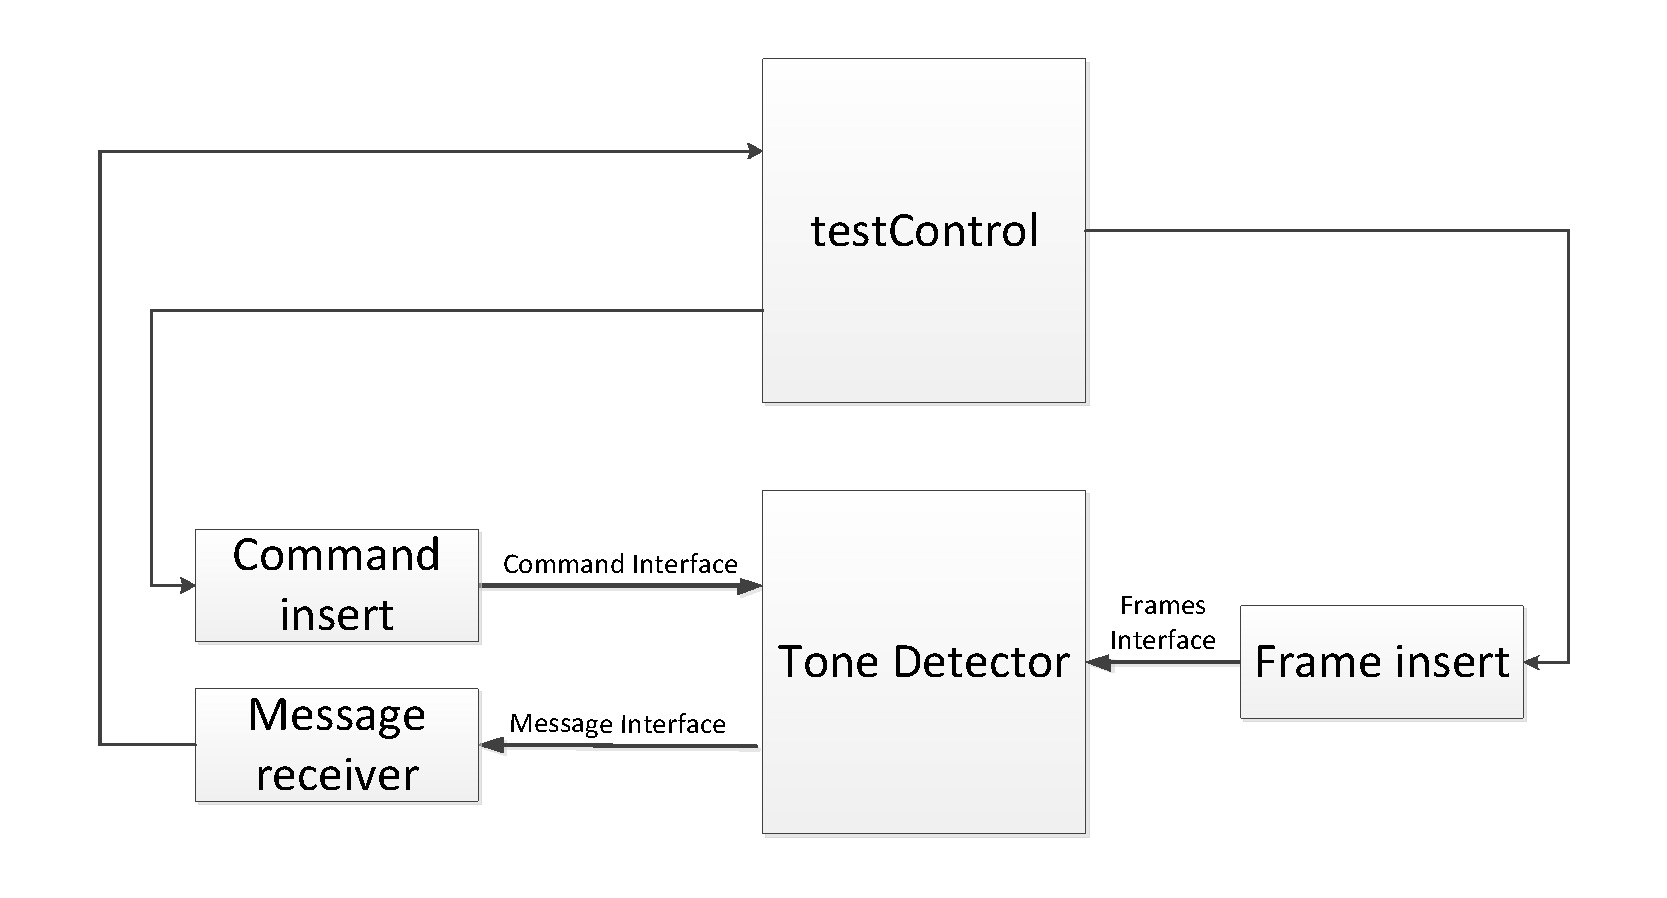
\includegraphics[scale=0.55]{img/modulos/mod_testControl.pdf}
				\caption{Test Unity}
				\label{fig:testUnityBlock}
				\end{figure}	

			A unidade de testes tem ciclo de execução orientado para os canais de processamento, ou seja, sua funcionalidade tem como base
			fazer com que os canais estejam sempre processando, enquanto houver áudios a serem processados. 

			Os áudios e os comando são gerados com uso de um programa desenvolvido em \textit{C ANSI}, o qual gera sinais com frequências, durações de pulsos,
			durações de pausas e valor de cadência com valores aleatórios, baseados nesses valores são calculados os parâmetros para cada áudio gerados.
			Este programa tem como saída os arquivos de áudios e o arquivo "fileParams.bin", que é um arquivos que contém
			os comandos para cada áudio gerado.
			Os valores das frequências estão dentro do intervalo $[400 Hz, 800 Hz]$. Os valores possíveis para as largura de pulsos e pausas estão no intervalo
			$[120 ms, 670 ms]$. Dentre os áudios gerados, $80\%$ não tem cadências, ou seja, o sinal não tem repetições, em $10\%$, a cadência tem valor um e nos
			outros $10\%$ a o sinal gerado tem cadência dois.

			O modelo funcional da unidade de testes está apresentado na Figura \ref{fig:testUnityFunctionalModel}, e nela estão apresentado os passos que 
			são seguidos pelo módulo controlador, por canal, para a simulação dos processamentos.

				\begin{figure}[!h]
				\centering
					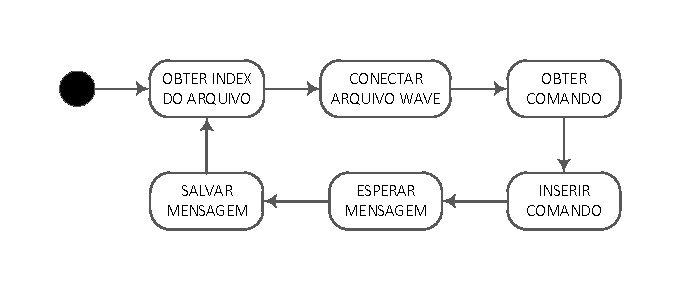
\includegraphics[scale=1.3]{img/stateMachines/unitTest.pdf}
				\caption{Test Unity Functional Model}
				\label{fig:testUnityFunctionalModel}
				\end{figure}

			A primeira etapa dos testes, \textit{GET FILE INDEX}, consiste em saber quais canais estão disponíveis para processamento, para isso, existe um
			array de 8 bits, para qual, cada bit representa se a porta está em uso, ou não, nível lógico alto significa canal disponível, e nível
			lógico baixo significa canal ocupado.
			
			Com a obtenção da informação de qual arquivo será utilizado, inicia-se a segunda etapa dos testes, a conexão do arquivo ao 
			\textit{Tone Detector}, através do módulo \textit{frameInserter}, que faz a leitura de um arquivos no formato ".wav", descartando apenas seu
			cabeçalho, e inserindo frames a uma frequência de $8Khz$.

			Depois de realizada a conexão do arquivo de áudio ao \textit{Tone Detector}, é utilizado seu index para a leitura do comando dentro do arquivo 
			"fileParams.bin", que contém os parâmetros para cada sinal gerado. Depois de lidos os parâmetros do áudio, é inserido o comando através do módulo
			\textit{commandInserter}. Esta são, respectivamente as etapas três e quatro.

			Após a etapa quatro, ou seja, a inserção do comando relativo ao áudio no canal, é dado início ao processamento. A tarefa da unidade de testes, para este
			canal, é ficar no aguardo pela mensagem da detecção, que consiste na etapa cinco. Com a chegada desta mensagem, seu conteúdo é salvo em um arquivo
			juntamente com a informação de index do arquivo e o valor da canal de processamento. Estas ações correspondem, respectivamente às etapas cinco e 
			seis da
			unidade de testes.

			Os processos realizados pela unidade de testes, verificação de canal livre, conexão de áudio, inserção dos comandos e recebimento das mensagens,
			são executados para cada canal de	detecção, e este ciclo é repetido até que todos os áudios gerados sejam processados.

\end{document}
